Our case of study focuses on a three-wheeled omnidirectional mobile robot which is a holonomic robot that has the ability to move simultaneously and independently in translation and rotation. The robot has three omni-wheels equally disposed at $120^\circ$, and have a distance $L$ from their center and the robot's center of mass $R \equiv O_m$.  

\begin{figure}[ht]
  \centering
  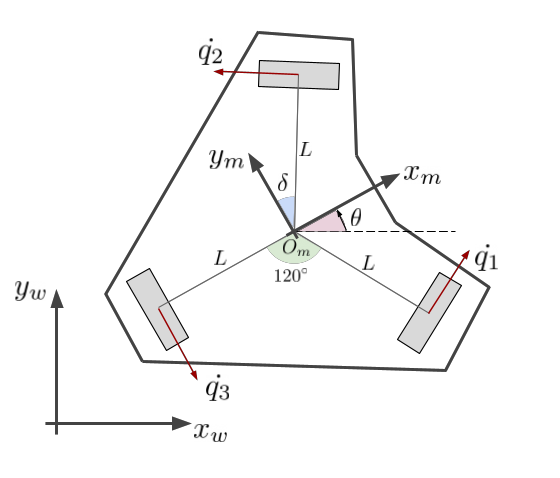
\includegraphics
      [width=0.35\textwidth]
      {figures/robot1.png}
  \caption{Three-wheeled omnidirectional mobile robot}
  \label{fig:robot_w}
\end{figure}

As shown in Fig. \ref{fig:robot_w}, there are two different reference frames: the first $RF_m \triangleq [O_m, X_m, Y_m]$ is a mobile frame placed at the robot's center of mass, the second one is the fixed world coordinate system $RF_w \triangleq [O_w, X_w, Y_w]$. Robot orientation w.r.t to $RF_w$ is given by the angle $\theta$. The angle $\delta$ is equal to $30^\circ$ and indicates the wheel orientation w.r.t. $RF_m$.

The kinematic model w.r.t. $RF_w$ is deduced as follows:

\begin{align}
    \dot{x} &= \begin{bmatrix}
           \frac{2}{3}\cos{(\theta + \delta)} & -\frac{2}{3}\cos{(\theta - \delta)} &  \frac{2}{3}\sin{\theta}   \\
           \frac{2}{3}\sin{(\theta + \delta)} & -\frac{2}{3}\sin{(\theta - \delta)} &  -\frac{2}{3}\cos{\theta} \\
           \frac{1}{3L} & \frac{1}{3L} & \frac{1}{3L}
         \end{bmatrix} \dot{q} 
  \label{eq:kin_model}
\end{align}
\begin{align*}
    &+ \begin{bmatrix}
         -sin{\theta} \\
         cos{\theta} \\
         0
        \end{bmatrix} d
\end{align*}

Where system state is given by $x = [^w x_R, ^w y_R, \theta]^T$. The second term represents an external disturbance given by a velocity with module $d$ and perpendicular to robot orientation $\theta$ (i.e. it lies on $Y_m$). The procedure to calculate (\ref{eq:kin_model}) is shown in the Appendix.

\begin{comment}
In this equation we can see a term multiplied by $d$, this term represents an introduced disturbance in the System. $\delta$ instead represents the orientation of the three wheels.So now we know that the reach-avoid set $RAS^\pm$ is described by the zero sublevel of the game's outcome $V^\pm(x,t)$. So given the model $f(x,u,d)$: 
\begin{equation*}
\begin{split}
f(\cdot) &= \\ \begin{pmatrix}
    \frac{2}{3}\cos{(\theta + \delta)}u_{1} - \frac{2}{3}\cos{(\theta - \delta)}u_{2} +\frac{2}{3}\sin{(\theta)}u_{3} - \sin{(\theta)d
    _{1}} \\
    \frac{2}{3}\sin{(\theta + \delta)}u_{1} - \frac{2}{3}\sin{(\theta - \delta)}u_{2} -\frac{2}{3}\cos{(\theta)}u_{3} - \cos{(\theta)}d
    _{2} \\
     \frac{1}{3L}u_{1} + \frac{1}{3L}u_{2} + \frac{1}{3L}u_{3}
\end{pmatrix}
\end{split}
\end{equation*}

The upper Hamiltonian is here:

\begin{equation}
    H^{*}(x,p) = \min_{u}\max_{d}(P_{1},P_{2},P_{3})f(x,u,d)
\end{equation}


So that $H^{*}$ becomes:
\begin{equation}
    \begin{split}
    H^{*} = \min_{u}\max_{d} &\begin{pmatrix}\frac{2}{3}\cos{(\theta + \delta)}P_{1} +  \frac{2}{3}\sin{(\theta + \delta)}P_{2} + \frac{1}{3L}P_{3}
    \end{pmatrix}u_{1} \\
    +  &\begin{pmatrix}-\frac{2}{3}\cos{(\theta -\delta)}P_{1} -\frac{2}{3}\sin{(\theta -\delta)}P_{2} + \frac{1}{3L}P_{3} \end{pmatrix}u_{2} \\
    +  &\begin{pmatrix}-\frac{2}{3}\sin{(\theta)}P_{1} -\frac{2}{3}\cos{(\theta)}P_{2} + \frac{1}{3L}P_{3} \end{pmatrix}u_{3} \\
    + &(-\sin{(\theta)}P_{1})d_{1}
    \\
    +&(\cos{(\theta)}P_{2})d_{2}
    \end{split}
\end{equation}


Here we can define $u_{1}$, $u_{2}$ and $u_{3}\in[U_{min}, U_{max}]$. We can choose here $U_{min}=-U_{max}$ to get the optimal control inputs so that:
    \begin{equation*}
    \begin{split}
        u^{*}_{1} &=\min_{u_{1}}\begin{pmatrix}\frac{2}{3}\cos{(\theta +  \delta)}P_{1} +  \frac{2}{3}\sin{(\theta + \delta)}P_{2} + \frac{1}{3L}P_{3}\end{pmatrix}u_{1} \\
         &=\min_{u_{1}}\gamma_{1}u_{1}
    \end{split}
    \end{equation*}
    \begin{equation}
    u^{*}_{1}=\begin{cases}
      U_{min}\quad \textrm{if} \quad \gamma_{1} \geq 0 \\
      U_{max}\quad \textrm{if} \quad \gamma_{1} < 0
    \end{cases}
\end{equation}
\\
    \begin{equation*}
    \begin{split}
        u^{*}_{2} &=\min_{u_{2}}\begin{pmatrix}-\frac{2}{3}\cos{(\theta -\delta)}P_{1} -\frac{2}{3}\sin{(\theta -\delta)}P_{2} + \frac{1}{3L}P_{3} \end{pmatrix}u_{2} \\
         &=\min_{u_{2}}\gamma_{2}u_{2}
        \end{split}
    \end{equation*}
    \begin{equation}
    u^{*}_{2}=\begin{cases}
      U_{min}\quad \textrm{if} \quad \gamma_{2} \geq 0 \\
      U_{max}\quad \textrm{if} \quad \gamma_{2} < 0
    \end{cases}
\end{equation}
%\\
    \begin{equation*}
    \begin{split}
        u^{*}_{3} &=\min_{u_{3}}\begin{pmatrix}-\frac{2}{3}\sin{(\theta)}P_{1} -\frac{2}{3}\cos{(\theta)}P_{2} + \frac{1}{3L}P_{3} \end{pmatrix}u_{3} \\
         &=\min_{u_{3}}\gamma_{3}u_{3}
        \end{split}
    \end{equation*}
    \begin{equation}
    u^{*}_{3}=\begin{cases}
      U_{min}\quad \textrm{if} \quad \gamma_{3} \geq 0 \\
      U_{max}\quad \textrm{if} \quad \gamma_{3} < 0
    \end{cases}
\end{equation}

\end{comment}
%\\
%\newpage

